\setcounter{chapter}{0}
\setcounter{section}{0}
\begin{center}
\chapter{\tenchuongi}
\end{center}

%===================================================================
\section{Khái quát về CNN}
\subsection{Giới thiệu}
Tương tự như việc trẻ em học cách nhận diện đối tượng, chúng ta cần cho thuật toán học rất nhiều hình ảnh trước khi nó có thể đưa ra phân loại cho hình ảnh đầu vào mà nó chưa từng thấy \cite{ntt8b3}.

\begin{figure}[H]
	\centering
	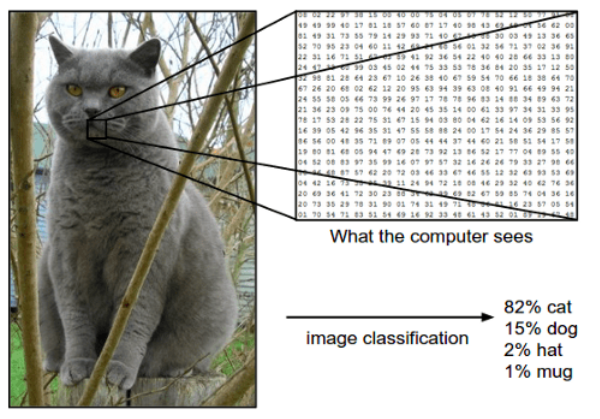
\includegraphics[width=0.7\linewidth]{images/how_computer_see_image}
	\caption[Cách máy tính "nhìn" một hình.]{Cách máy tính "nhìn" một hình.}
	%\label{fig:howcomputerseeimage}
\end{figure}

Máy tính “nhìn” theo cách khác con người. Trong thế giới máy tính chỉ có những con số. Mỗi hình ảnh có thể được biểu diễn dưới dạng mảng 2 chiều những con số được gọi là các pixel.

Mặc dù máy tính nhìn nhận theo cách khác con người, chúng ta vẫn có thể dạy máy tính nhận diện các mẫu như con người. Điều quan trọng là chúng ta cần nghĩ về hình ảnh theo một cách khác đi.

Để dạy thuật toán nhận diện đối tượng trong hình ảnh, ta sử dụng một loại mạng ANN, đó là CNN. Tên của nó được dựa trên phép tính quan trọng được sử dụng trong mạng- tích chập.

Mạng CNN lấy cảm hứng từ não người. Nghiên cứu trong những thập niên 1950 và 1960 của D.H Hubel và T.N Wiesel trên não của động vật đã đề xuất một mô hình mới cho việc cách mà động vật nhìn nhận thế giới. Trong báo cáo, hai ông đã diễn tả 2 loại tế bào nơ-ron trong não và cách hoạt động khác nhau: tế bào đơn giản (simple cell – S cell) và tế bào phức tạp (complex cell – C cell). 

Các tế bào đơn giản được kích hoạt khi nhận diện các hình dáng đơn dản như đường nằm trong một khu vực cố định và một góc cạnh của nó. Các tế bào phức tạp có vùng tiếp nhận lơn hơn và đầu ra của nó không nhạy cảm với những vị trí cố định trong vùng. 

Trong thị giác, vùng tiếp nhận của một nơ-ron tương ứng với một vùng trên võng mạc nơi mà sẽ kích hoạt nơ-ron tương ứng. 

Năm 1980, Fukushima đề xuất mô hình mạng nơ-ron có cấp bậc gọi là neocognitron. Mô hình này dựa trên khái niệm về S cell và C cell. Mạn neocognitron có thể nhận diện mẫu dựa trên việc học hình dáng của đối tượng. 

Sau đó vào năm 1998, mạng CNN được giới thiệu bởi Bengio, Le Cun, Bottou và Haffner. Mô hình đầu tiên của họ được gọi tên là LeNet-5. Mô hình này có thể nhận diện chữ số viết tay.

\subsection{Kiến trúc mạng CNN}
Mạng CNN có kiến trúc khác với Mạng Nơ-ron thông thường. Mạng ANN bình thường chuyển đổi đầu vào thông qua hàng loạt các tầng ẩn. Mỗi tầng là một tập các nơ-ron và các tầng được liên kết đầy đủ với các nơ-ron ở tầng trước đó. Và ở tầng cuối cùng sẽ là tầng kết quả đại diện cho dự đoán của mạng.

Đầu tiên, mạng CNN được chia thành 3 chiều: rộng, cao, và sâu. Kế đến, các nơ ron trong mạng không liên kết hoàn toàn với toàn bộ nơ-ron lớp sau mà chỉ liên kết tới một vùng nhỏ. Cuối cùng, một tầng đầu ra được tối giản thành véc-tơ của giá trị xác suất (hình \ref{fig:neuronnetwork}).

\begin{figure}[H]
	\centering
	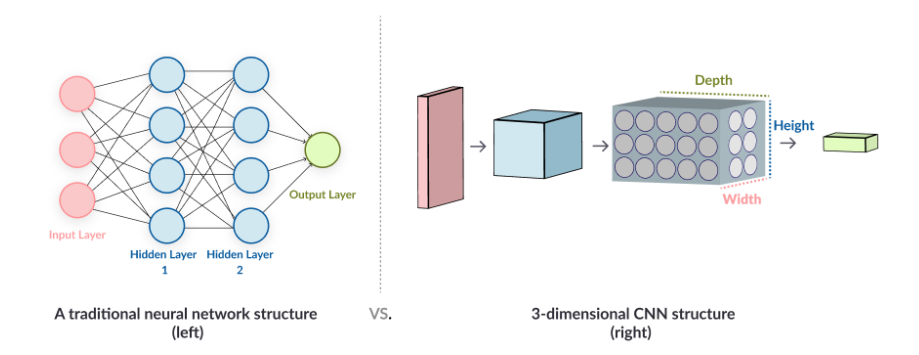
\includegraphics[width=1\linewidth]{images/neuronnetwork}
	\caption{Mạng Neuron thông thường (trái) và CNN (phải).}
	\label{fig:neuronnetwork}
\end{figure}

Mạng CNN gồm hai thành phần:

\indent\indent \textbf{Phần tầng ẩn hay phần rút trích đặc trưng:} trong phần này, mạng sẽ tiến hành tính toán hàng loạt phép tích chập và phép hợp nhất (pooling) để phát hiện các đặc trưng. Ví dụ: nếu ta có hình ảnh con ngựa vằn, thì trong phần này mạng sẽ nhận diện các sọc vằn, hai tai, và bốn chân của nó.

\indent\indent  \textbf{Phần phân lớp:} tại phần này, một lớp với các liên kết đầy đủ sẽ đóng vai trò như một bộ phân lớp các đặc trưng đã rút trích được trước đó. Tầng này sẽ đưa ra xác suất của một đối tượng trong hình \ref{fig:kientruccnn}.
\begin{figure}[H]
	\centering
	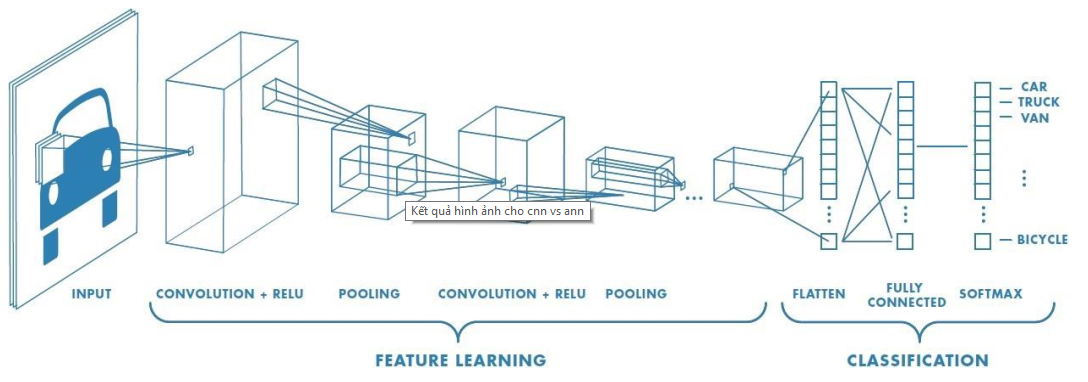
\includegraphics[width=1\linewidth]{images/kientruccnn}
	\caption{Kiến trúc mạng CNN.}
	\label{fig:kientruccnn}
\end{figure}

\subsubsection{Trích rút đặc trưng}
\paragraph{Lớp tích chập}
Tích chập là một khối quan trọng trong CNN. Thuật ngữ tích chập được dựa trên một phép hợp nhất toán học của hai hàm tạo thành hàm thứ ba. Phép toán này kết hợp hai tập thông tin khác nhau.

Trong trường hợp CNN, tích chập được thực hiện trên giá trị đầu vào của dữ liệu và kernel/filter (thuật ngữ này được sử dụng khác nhau tùy tình huống) để tạo ra một bản đồ đặc trưng (feature map). 

Ta thực hiện phép tích chập bằng cách trượt kernel/filter theo dữ liệu đầu vào. Tại mỗi vị trí, ta tiến hành phép nhân ma trận và tính tổng các giá trị để đưa vào bản đồ đặc trưng. Thao tác này đã được minh họa cụ thể trong hình \ref{fig:padding18}

\begin{figure}[H]
	\centering
	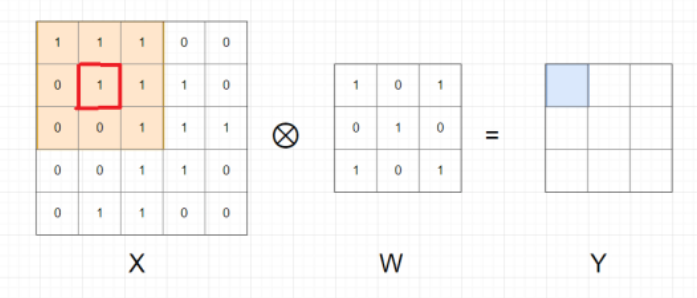
\includegraphics[width=1\linewidth]{images/padding18.png}
	\caption{Minh họa phép tích chập.}
	\label{fig:padding18}
\end{figure}

Trong thực tế, tích chập được thực hiện hiện trên không gian 3 chiều. Vì mỗi hình ảnh được biểu diễn dưới dạng 3 chiều: rộng, cao, và sâu. Chiều sâu ở đây chính là giá trị màu sắc của hình (RGB).

Ta thực hiện phép tích chập trên đầu vào nhiều lần khác nhau. Mỗi lần sử dụng một kernel/filter khác nhau. Kết quả ta sẽ thu được những bản đồ đặc trưng khác nhau. Cuối cùng, ta kết hợp toàn bộ bản đồ đặc trưng này thành kết quả cuối cùng của tầng tích chập.

\paragraph{Lớp ReLU}

Tương tự như mạng nơ-ron thông thường, ta sử dụng một hàm kích hoạt (activate function) để có đầu ra dưới dạng phi tuyến. Trong trường hợp CNN, đầu ra của phép tích chập sẽ đi qua hàm kích hoạt nào đó ví dụ như hàm tinh chỉnh các đơn vị tuyến tính (Rectified linear units - ReLU). 

Trong quá trình trượt kernel/filter trên dữ liệu đầu vào, ta sẽ quy định một bước nhảy (stride) với mỗi lần di chuyển. Thông thường ta lựa chọn thường chọn bước nhảy là 1. Nếu kích thước bước nhảy tăng, kernel/filter sẽ có ít ô trùng lắp.

Bởi vì kích thước đầu ra luôn nhỏ hơn đầu vào nên ta cần một phép xử lí đầu vào để đầu ra không bị co giãn. Đơn giản ta chỉ cần thêm một lề nhỏ vào đầu vào. Một lề (padding) với giá trị 0 sẽ được thêm vào xung quanh đầu vào trước khi thực hiện phép tích chập. 

\paragraph{Lớp pooling}

Thông thường, sau mỗi tầng tích chập, ta sẽ cho kết quả đi qua một tầng hợp nhất (pooling layer). Mục đích của tầng này là để nhanh chóng giảm số chiều. Việc này giúp giảm thời gian học và hạn chế việc overfitting. 

Một phép hợp nhất đơn giản thường được dùng đó là max pooling, phép này lấy giá trị lớn nhất của một vùng để đại diện cho vùng đó. Kích thước của vùng sẽ được xác định trước để giảm kích thước của bản đồ đặc trưng nhanh chóng nhưng vẫn giữ được thông tin cần thiết (hình \ref{fig:maxpooling22}).

\begin{figure}[H]
	\centering
	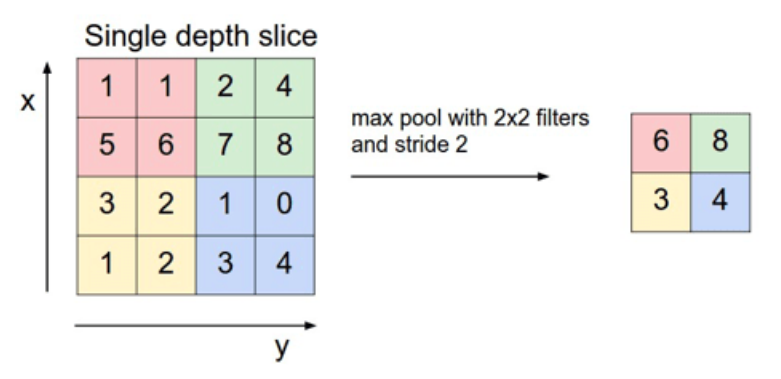
\includegraphics[width=0.8\linewidth]{images/maxpooling22.png}
	\caption{Max pooling kích thước 2×2}
	\label{fig:maxpooling22}
\end{figure}

Như vậy, khi thiết kế phần rút trích đặc trưng của mạng CNN, ta cần chú ý đến 4 siêu tham số quan trọng là: Kích thước kernel/filter, Số lượng kernel/filter, Kích thước bước nhảy (stride), Kích thước lề (padding).

\subsubsection{Phân lớp}
Trong phần phân lớp, ta sử dụng một vài tầng với kết nối đầy đủ để xử lí kết quả của phần tích chập. Vì đầu vào của mạng liên kết đầy đủ là 1 chiều, ta cần làm phẳng đầu vào trước khi phân lớp. Tầng cuối cùng trong mạng CNN là một tầng liên kết đầy đủ, phần này hoạt động tương tự như mạng nơ-ron thông thường.

Kết quả thu được cuối cùng cũng sẽ là một véc-tơ với các giá trị xác suất cho việc dự đoán như mạng nơ-ron thông thường.

\begin{figure}[H]
	\centering
	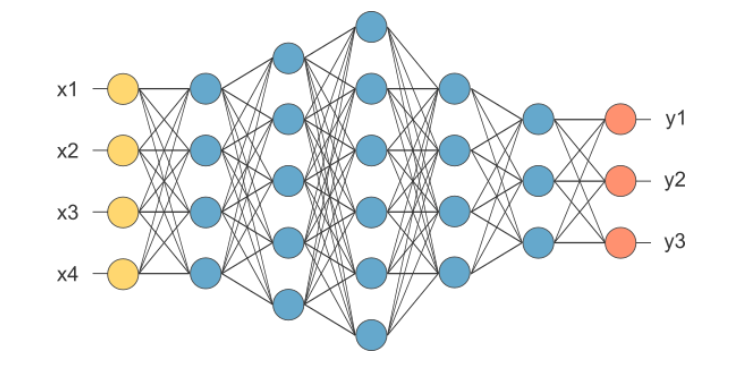
\includegraphics[width=0.8\linewidth]{images/fullyconnected.png}
	\caption{Lớp kết nối đầy đủ}
\end{figure}

\subsection{Ứng dụng CNN trong phân loại ảnh}
\begin{figure}[H]
	\centering
	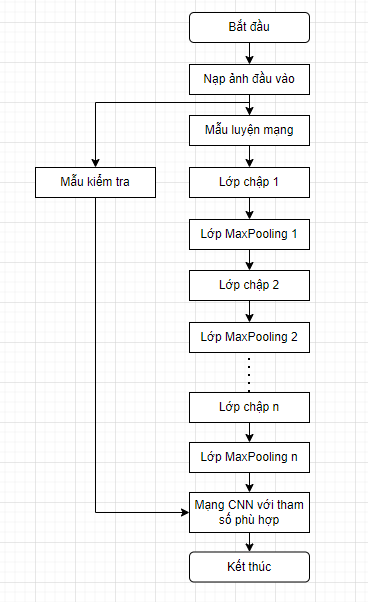
\includegraphics[width=0.8\linewidth]{images/placnn.png}
	\caption{Max pooling kích thước 2×2}
	\label{fig:placnn}
\end{figure}
Các bước để thực hiện phân loại hình ảnh dựa trên mạng CNN được mô tả trong Hình \ref{fig:placnn}. Đầu tiên, kho dữ liệu ảnh đầu vào được nạp. Ảnh này được chia làm hai phần, một phần dành cho luyện mạng và một phần cho kiểm tra. Trước tiên, ta phải lựa chọn cấu trúc mạng CNN bao gồm số lượng lớp ẩn, các tham số trong mỗi lớp ẩn như kích thước trường tiếp nhận cục bộ, stride, padding.  Ảnh luyện mạng sau đó được đưa vào lớp chập 1 để thực hiện tích chập trên ảnh và thực hiện hàm ReLU. Sau đó, kết quả được đưa đến quá trình thực hiện pooling với tham số pooling size phù hợp để giảm kích cỡ ảnh. Ảnh sẽ tiếp tục được đưa thêm qua các lớp tích chập nữa cho đến khi đạt được kết quả mong muốn. Kết quả này được dàn phẳng và đưa vào lớp kết nối đầy đủ. Cuối cùng là quá trình thực hiện các activation function và phân loại ảnh. Quá trình luyện mạng sẽ kết thúc sau khi tổng sai số nhỏ hơn một ngưỡng cho phép hoặc sau một số thế hệ cho trước (điều kiện hội tụ). Kết thúc của quá trình luyện mạng là cấu trúc mạng CNN với các tham số phù hợp. Để kiểm tra, các mẫu ảnh kiểm tra được đưa qua mạng CNN rồi thực hiện đánh giá sai số.

\subsection{Xây dựng mạng CNN cho phân loại ảnh}
Trước tiên, đối với mỗi điểm ảnh trong ảnh đầu vào, ta mã hóa cường độ của 
điểm ảnh là giá trị của nơron tương ứng trong tầng đầu vào.
 
Ví dụ đối với bài toán nhận dạng chữ viết tay từ tập dữ liệu MNIST, mỗi bức 
ảnh kích thước 28x28 điểm ảnh. Do vậy, mạng có 784 (28x28) nơron đầu vào (Hình 
\ref{fig:lopinput}). Sau đó ta huấn luyện trọng số (weight) và độ lệch (bias) để đầu ra của mạng 
như ta mong đợi là xác định chính xác ảnh các chữ số 0, 1, 2...8, 9.

Mạng tích chập sử dụng 3 ý tưởng cơ bản: các trường tiếp nhận cục bộ (local 
receptive field), trọng số chia sẻ (shared weights) và tổng hợp (pooling). Chúng ta 
hãy xem xét lần lượt từng ý tưởng.

\subsubsection{Trường tiếp nhận cục bộ (Local receptive fields)}
Như thường lệ chúng ta sẽ kết nối các điểm ảnh đầu vào cho các nơron ở tầng 
ẩn. Nhưng chúng ta sẽ không kết nối mỗi điểm ảnh đầu vào cho mỗi neuron ẩn. Thay 
vào đó, chúng ta chỉ kết nối trong phạm vi nhỏ, các vùng cục bộ của bức ảnh.
\begin{figure}[H]
	\centering
	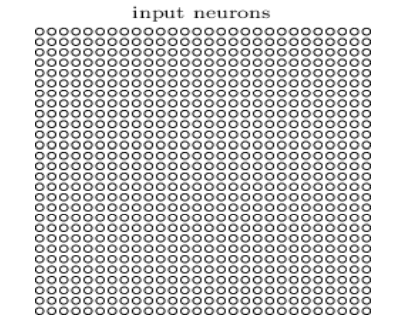
\includegraphics[width=0.5\linewidth]{images/lopinput.png}
	\caption{Lớp input gồm 28x28 nơ ron cho nhận dạng chữ từ tập dữ liệu MNIST}
	\label{fig:lopinput}
\end{figure}
Để được chính xác hơn, mỗi nơron trong lớp ẩn đầu tiên sẽ được kết nối với 
một vùng nhỏ của các nơron đầu vào, ví dụ, một vùng 5 × 5, tương ứng với 25 điểm ảnh đầu vào. Vì vậy, đối với một nơron ẩn cụ thể, chúng ta có thể có các kết nối như Hình \ref{fig:ketnoivung} sau:
\begin{figure}[H]
	\centering
	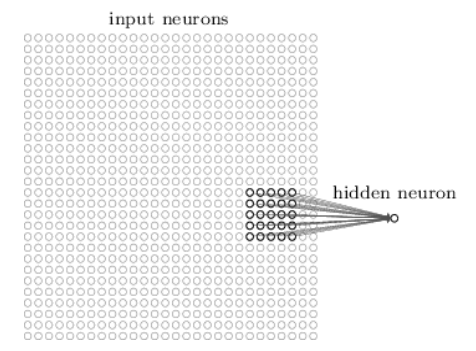
\includegraphics[width=0.6\linewidth]{images/ketnoivung.png}
	\caption{Kết nối vùng 5x5 neuron input với nơ ron lớp ẩn}
	\label{fig:ketnoivung}
\end{figure}
Vùng đó trong bức ảnh đầu vào được gọi là vùng tiếp nhận cục bộ cho nơron 
ẩn. Đó là một cửa sổ nhỏ trên các điểm ảnh đầu vào. Mỗi kết nối sẽ học một trọng số
và nơron ẩn cũng sẽ học một độ lệch (overall bias). Ta có thể hiểu rằng, nơron lớp ẩn 
cụ thể học để phân tích trường tiếp nhận cục bộ cụ thể của nó.

Sau đó chúng ta trượt trường tiếp nhận cục bộ trên toàn bộ bức ảnh. Đối với 
mỗi trường tiếp nhận cục bộ, có một nơron ẩn khác trong tầng ẩn đầu tiên. Để minh 
họa điều này một cách cụ thể, chúng ta hãy bắt đầu với một trường tiếp nhận cục 
bộ ở góc trên bên trái (Hình \ref{fig:truongtiepnhancucbo}):
\begin{figure}[H]
	\centering
	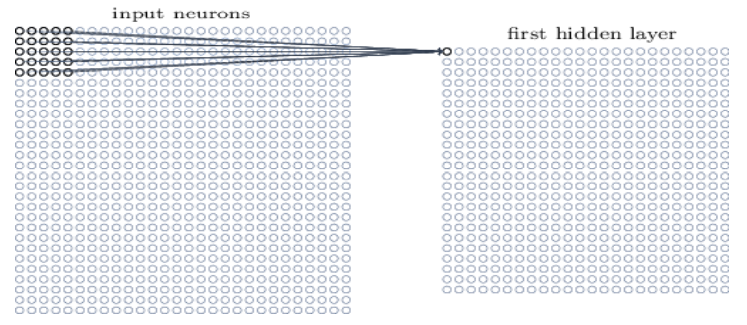
\includegraphics[width=1\linewidth]{images/truongtiepnhancucbo.png}
	\caption{Vị trí bắt đầu của trường tiếp nhận cục bộ}
	\label{fig:truongtiepnhancucbo}
\end{figure}
Sau đó, chúng ta trượt trường tiếp nhận cục bộ trên bởi một điểm ảnh bên 
phải (tức là bằng một nơron), để kết nối với một nơron ẩn thứ hai (Hình \ref{fig:truongtiepnhancucbo2}):
\begin{figure}[H]
	\centering
	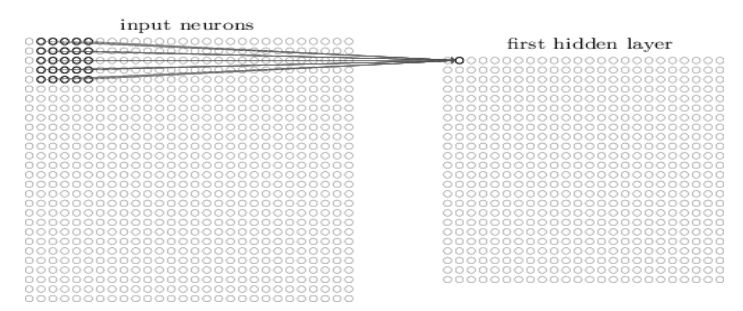
\includegraphics[width=1\linewidth]{images/truongtiepnhancucbo2.png}
	\caption{Vị trí thứ 2 của trường tiếp nhận cục bộ và neuron lớp ẩn}
	\label{fig:truongtiepnhancucbo2}
\end{figure}
Cứ như vậy, ta sẽ xây dựng các lớp ẩn đầu tiên. Lưu ý rằng nếu chúng ta có một ảnh đầu vào 28 × 28 và 5 × 5 trường tiếp nhận cục bộ thì ta sẽ có 24 × 24 nơron trong lớp ẩn. Có được điều này là do chúng ta chỉ có thể di chuyển các trường tiếp nhận cục bộ ngang qua 23 nơron (hoặc xuống dưới 23 nơron), trước khi chạm với phía bên phải (hoặc dưới) của ảnh đầu vào.
 
Với bài toán nhận dạng ảnh người ta thường gọi ma trận lớp ẩn đầu vào là feature map, trọng số xác định các đặc trưng là shared weight và độ lệch xác định một feature map là shared bias. Như vậy đơn giản nhất là qua các bước trên chúng ta chỉ có 1 feature map. Tuy nhiên trong nhận dạng ảnh chúng ta cần nhiều hơn một feature map.
\begin{figure}[H]
	\centering
	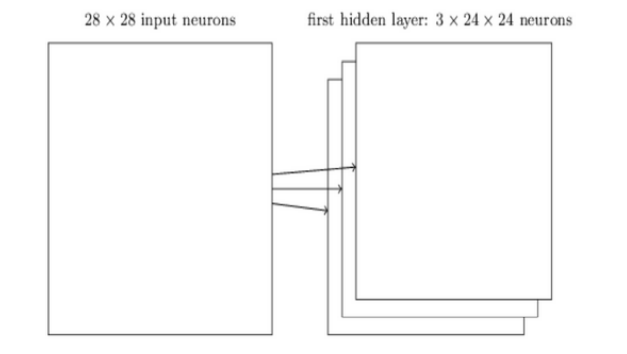
\includegraphics[width=0.8\linewidth]{images/babandodactrung.png}
	\caption{Trường tiếp nhận cục bộ với ba bản đồ đặc trưng}
	\label{fig:babandodactrung}
\end{figure}
Trong ví dụ ở Hình \ref{fig:babandodactrung}, có 3 bản đồ đặc trưng. Mỗi bản đồ đặc trưng được xác định bởi một tập 5 × 5 trọng số chia sẻ, và một độ lệch chia sẻ duy nhất. Kết quả là các mạng có thể phát hiện 3 loại đặc trưng khác nhau, với mỗi đặc trưng được phát hiện trên toàn bộ ảnh. 

Trong thực tế mạng CNN có thể sử dụng nhiều bản đồ đặc trưng hơn. Một trong những mạng chập đầu tiên là LeNet-5, sử dụng 6 bản đồ đặc trưng, mỗi bản đồ được liên kết đến một trường tiếp nhận cục bộ 5 × 5, để phát hiện các kí tự MNIST. Vì vậy, các ví dụ minh họa ở trên là thực sự khá gần LeNet-5. Trong một số nghiên cứu gần đây sử dụng lớp tích chập với 20 và 40 bản đồ đặc trưng.
\begin{figure}[H]
	\centering
	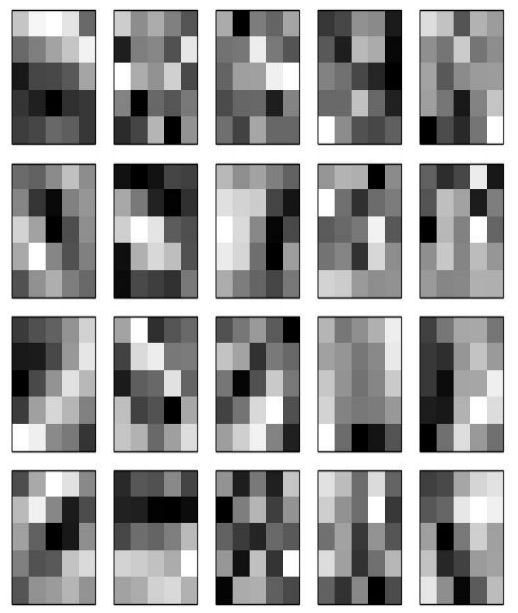
\includegraphics[width=0.8\linewidth]{images/20bandodactrung.png}
	\caption{Trường tiếp nhận cục bộ với 20 bản đồ đặc trưng}
	\label{fig:20bandodactrung}
\end{figure}
Trên đây (hình \ref{fig:20bandodactrung}) là 20 ảnh tương ứng với 20 bản đồ đặc trưng khác nhau (hay còn gọi là bộ lọc, hay là nhân). Mỗi bản đồ được thể hiện là một hình khối kích thước 5 × 5, tương ứng với 5 × 5 trọng số trong trường tiếp nhận cục bộ. Khối trắng có nghĩa là một trọng số nhỏ hơn, vì vậy các bản đồ đặc trưng đáp ứng ít hơn để tương ứng với điểm ảnh đầu vào. Khối sẫm màu hơn có nghĩa là trọng số lớn hơn, do đó, các bản đồ đặc trưng đáp ứng nhiều hơn với các điểm ảnh đầu vào tương ứng.

Có thể thấy rằng, trường tiếp nhận cục bộ thích hợp cho việc phân tách dữ liệu ảnh, giúp chọn ra những vùng ảnh có giá trị nhất cho việc đánh giá phân lớp.

\subsubsection{Trọng số chia sẻ và độ lệch (Shared weights and biases)}
Đầu tiên, các trọng số cho mỗi filter (kernel) phải giống nhau. Tất cả các nơ-ron trong lớp ẩn đầu sẽ phát hiện chính xác feature tương tự chỉ ở các vị trí khác nhau trong hình ảnh đầu vào. Chúng ta gọi việc map từ input layer sang hidden layer là một feature map. Ta cần tìm ra mối quan hệ giữa số lượng Feature map với số lượng tham số.

Chúng ta thấy mỗi fearture map cần 25 = 5×5 shared weight và 1 shared bias. Như vậy mỗi feature map cần 5×5+1 = 26 tham số. Như vậy nếu có 10 feature map thì có 10×26 = 260 tham số. Chúng ta xét lại nếu layer đầu tiên có kết nối đầy đủ nghĩa là chúng ta có 28×28=784 neuron đầu vào như vậy ta chỉ có 30 neuron ẩn. Như vậy ta cần 28x28x30 shared weight và 30 shared bias. Tổng số tham số là 
28x28x30+30 tham số lớn hơn nhiều so với CNN. Ví dụ vừa rồi chỉ mô tả để thấy được sự ước lượng số lượng tham số chứ chúng ta không so sánh được trực tiếp vì 2 mô hình khác nhau. Nhưng điều chắc chắn là nếu mô hình có số lượng tham số ít hơn thì nó sẽ chạy nhanh hơn.

\subsubsection{Lớp chứa hay lớp tổng hợp (Pooling layer)}
Ngoài các lớp tích chập vừa mô tả, mạng nơron tích chập cũng chứa các lớp pooling. Lớp pooling thường được sử dụng ngay sau lớp tích chập. Những gì các lớp pooling làm là đơn giản hóa các thông tin ở đầu ra từ các lớp tích chập. 

Ví dụ, mỗi đơn vị trong lớp pooling có thể thu gọn một vùng 2 × 2 nơron trong lớp trước. Một thủ tục pooling phổ biến là max-pooling. Trong maxpooling, một đơn vị pooling chỉ đơn giản là kết quả đầu ra kích hoạt giá trị lớn nhất trong vùng đầu vào 2 × 2, như minh họa trong hình \ref{fig:cnnmaxpooling22} sau: 
\begin{figure}[H]
	\centering
	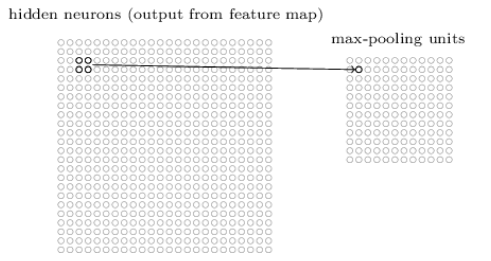
\includegraphics[width=0.8\linewidth]{images/cnnmaxpooling22.png}
	\caption{Trường tiếp nhận cục bộ với 20 bản đồ đặc trưng}
	\label{fig:cnnmaxpooling22}
\end{figure}
Lưu ý rằng bởi vì chúng ta có 24 × 24 nơron đầu ra từ các lớp tích chập, sau khi pooling chúng ta có 12 × 12 nơron.

Như đã đề cập ở trên, lớp tích chập thường có nhiều hơn một bản đồ đặc trưng. Chúng ta áp dụng max-pooling cho mỗi bản đồ đặc trưng riêng biệt. Vì vậy, nếu có ba bản đồ đặc trưng, các lớp tích chập và max-pooling sẽ kết hợp như hình \ref{fig:maxpoolingvoibabandodactrung} sau:
\begin{figure}[H]
	\centering
	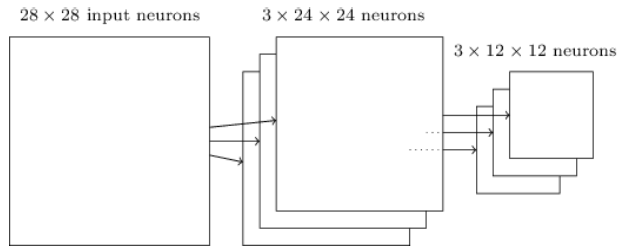
\includegraphics[width=0.8\linewidth]{images/maxpoolingvoibabandodactrung.png}
	\caption{Trường tiếp nhận cục bộ với 20 bản đồ đặc trưng}
	\label{fig:maxpoolingvoibabandodactrung}
\end{figure}
Chúng ta có thể hiểu max-pooling như là một cách cho mạng để hỏi xem một đặc trưng nhất được tìm thấy ở bất cứ đâu trong một khu vực của ảnh. Sau đó nó bỏ đi những thông tin định vị chính xác. Trực giác là một khi một đặc trưng đã được tìm thấy, vị trí chính xác của nó là không quan trọng như vị trí thô của nó so với các đặc trưng khác. Một lợi ích lớn là có rất nhiều tính năng gộp ít hơn (fewer pooled features), và vì vậy điều này sẽ giúp giảm số lượng các tham số cần thiết trong các lớp sau.

Max-pooling không phải là kỹ thuật duy nhất được sử dụng để pooling. Một phương pháp phổ biến khác được gọi là L2 pooling. Ở đây, thay vì lấy giá trị kích hoạt tối đa (maximum activation) của một vùng 2 × 2 nơron, chúng ta lấy căn bậc hai của tổng các bình phương của kích hoạt trong vùng 2 × 2. Trong khi các chi tiết thì khác nhau, nhưng về trực giác thì tương tự như max-pooling: L2 pooling là một cách để cô đọng thông tin từ các lớp tích chập. Trong thực tế, cả hai kỹ thuật đã được sử dụng rộng rãi. Và đôi khi người ta sử dụng các loại pooling khác.

Như vậy, chúng ta có thể đặt tất cả những ý tưởng lại với nhau để tạo thành một mạng tích chập hoàn chỉnh. Nó tương tự như kiến trúc chúng ta phân tích ở trên, nhưng có thêm một lớp 10 nơron đầu ra, tương ứng với 10 giá trị có thể cho các số MNIST ('0', '1', '2', v.v…) (hình \ref{fig:cnnnhandangchuviet}):
\begin{figure}[H]
	\centering
	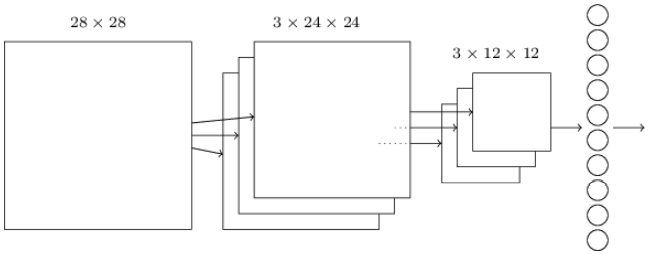
\includegraphics[width=1\linewidth]{images/cnnnhandangchuviet.png}
	\caption{Một kiến trúc mạng CNN cho nhận dạng chữ viết từ dữ liệu MNIST}
	\label{fig:cnnnhandangchuviet}
\end{figure}
Mạng bắt đầu với 28 × 28 nơron đầu vào, được sử dụng để mã hóa các cường độ điểm ảnh cho ảnh MNIST. Sau đó là một lớp tích chập sử dụng 5 × 5 trường tiếp nhận cục bộ và 3 bản đồ đặc trưng. Kết quả là một lớp 3 × 24 × 24 nơron lớp ẩn. Bước tiếp theo là một lớp max-pooling, áp dụng cho 2 × 2 vùng qua 3 bản đồ đặc trưng (feauture maps). Kết quả là một lớp 3 × 12 × 12 nơron đặc trưng ở tầng ẩn.

Lớp cuối cùng của các kết nối trong mạng là một lớp đầy đủ kết nối. Lớp này nối mọi nơron từ lớp max-pooled tới mọi nơron của tầng ra.

\subsubsection{Cách chọn tham số cho CNN}
Hiệu quả hoạt động của mạng CNN phụ thuộc rất nhiều vào việc lựa chọn các tham số sau:

\begin{itemize}
	\item Số các convolution layer: càng nhiều các convolution layer thì performance càng được cải thiện. Sau khoảng 3 hoặc 4 layer, các tác động được giảm một cách đáng kể.
	\item Filter size: thường filter theo size 5×5 hoặc 3×3
	\item Pooling size: thường là 2×2 hoặc 4×4 cho ảnh đầu vào lớn
\end{itemize}

Trong thực tế, tùy vào ứng dụng cụ thể mà ta chọn các tham số khác nhau. Thông thường ta sẽ thực hiện nhiều lần việc train test để chọn ra được param tốt nhất (Phương pháp thử sai).

\section{Bài toán chuẩn đoán bệnh lao}